\documentclass[A4paper, 11pt]{article}
\usepackage[slovene]{babel}
\usepackage[utf8]{inputenc}
\usepackage{graphicx}
\graphicspath{ {slike/} }

\title{Kodiranje s pomočjo sudoku ključa}
\author{Klementina Pirc}
\date{26.04.2018}

\newtheorem{definicija}{Definicija}


\begin{document}

\maketitle


% UVOD

\section{Uvod}

V današnjem svetu, kjer se vsak dan preko različnih komunikacijskih kanalov pretoči nepredstavljiva količina informacij, se pojavi vprašanje varovanja osebnih podatkov. Tema je še posebej aktualna na področju spletnih bančnih storitev in drugih podobno zaupnih dejavnostih. Pomagamo si s šifriranjem podatkov, navadno s pomočjo neke metode ali ključa, ki ga pozna le prejemnik in ga nato uporabi za dešifriranje prejetega sporočila. Pri šifriranju s ključem naletimo na problem, kako ključ za dešifriranje na varen način in v realnem času sporočiti našemu sogovorniku. Če namreč prisluškovalec prestreže naš ključ in za tem še sporočilo, bo brez težav dešifriral podatke. [2]

Kvantno šifriranje oziroma kvantna kriptografija temelji na posebnih fizikalnih lastnosti svetlobnih delcev - fotonov. Te lastnostii omogočajo varen prenos šifrirnega ključa tudi preko javnega, nezaščitenega komunikacijskega kanala. Še več, s pomočjo te metode lahko celo ugotovimo, ali je bila med pošiljateljem in prejemnikom prisotna tretja oseba, torej prisluškovalec in po potrebi pripravimo nov ključ za šifriranje. [2]


%POLARIZACIJA FOTONOV

\section{Polarizacija fotonov}


%BB84 PROTOKOL

\section{BB84 protokol}


%KVANTNA RAZDELITEV KLJUČA

\section{Kvantna razdelitev ključa}


%SUDOKU

\section{Sudoku}

\begin{definicija} %beamer
Sudoku je logična uganka, pri kateri je cilj zapolniti mrežo velikosti 9x9 s števili od 1 do 9 tako, da se vsako število v vsakem stolpcu, vrstici in 3x3 kvadratu znotraj mreže pojavi natanko enkrat. [3]
\end{definicija}

\begin{figure}[h] %beamer
\centering
\caption{Primer rešenega sudokuja}
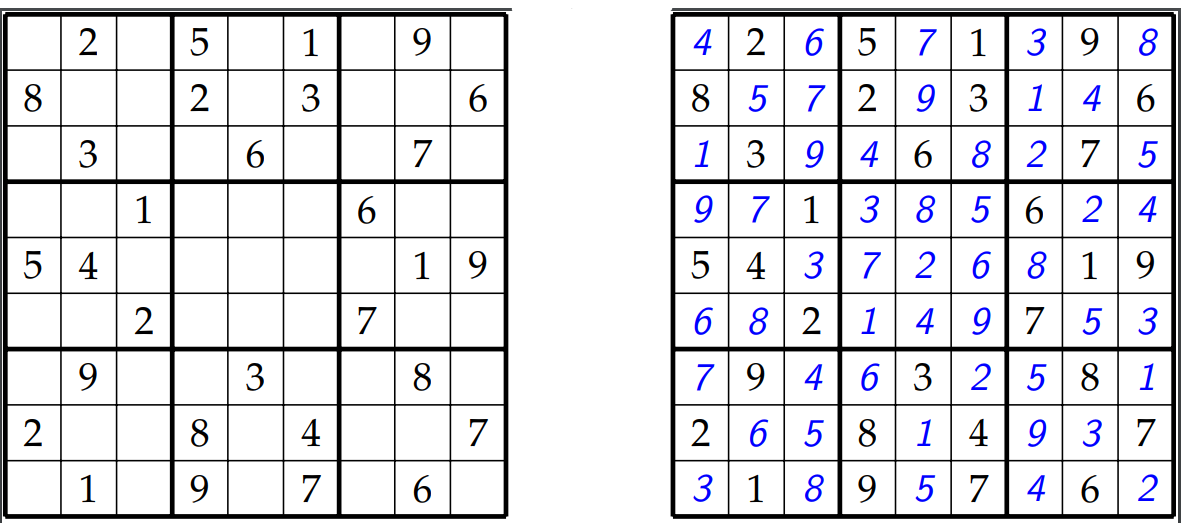
\includegraphics[scale=0.4]{sudoku_resen}
\end{figure}

Sudokuja se je domislil američan Howard Garns in ga prvič objavil leta 1979. Pravijo, da idejo dobil na podlagi Eulerjevega latinskega kvadrata. To je matrika velikosti nxn, napolnjena z n različnimi znaki, pri čemer se vsak znak v vrstici in stolpcu pojavi natanko enkrat. Čez 5 let so uganko objavili tudi na Japonskem in jo poimenovali ''Suuji wa dokushin ni kagiru'', kar v prevodu pomeni ''števke morajo biti edine'', prvi zlogi besed pa nam podajo ravno znano ime uganke: SUDOKU. [3]

%primer latinskega kvadrata na tablo
%poveš da je triljov 10 na 21

Število vseh možnih sudoku mrež, pri velikosti 9x9 je približno 6,6 trilijonov natančneje 6.670.903.752.021.072.936.960. 
Zahtevnost uganke je obratno sorazmerna s številom že vpisanih števil. Lažji sudokuji imajo tako podanih več kot 30 števil, težji pa nekje med 20 in 30. Dolgo je bil odprt problem najmanjšega števila začetnih števil, ki še vedno podajo enolično rešitev. Leta 2012 so dokazali, da je to število 17, saj za sistem s 16 podanimi števili niso našli rešitve. [3]

Skozi leta so se razvile različne oblike sudokujev in prispevale k težavnosti reševanja. Poznamo naprimer Sudoku X, pri katerem mora poleg standardnih pogojev veljati še, da se števila tudi na diagonalah pojavijo le enkrat. Še bolj ekstremna oblika pa je geometrijski sudoku, pri katerem znotraj mreže nimamo 3x3 kvadratov, temveč različne geometrijske like sestavljene iz devetih polj. [3]

\begin{figure}[h]
\centering
\caption{Geometrijski sudoku}
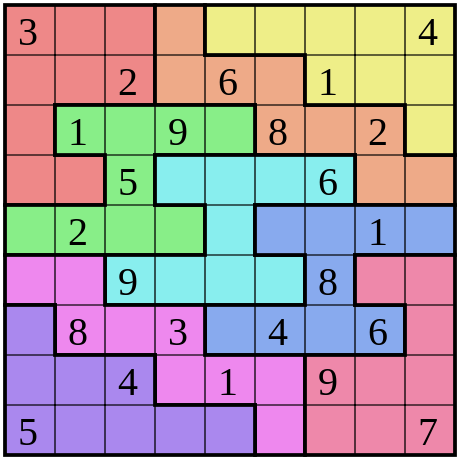
\includegraphics[scale=0.4]{geo_sudoku}
\end{figure}


\section{Sudoku ključ}

\end{document}
